\section{A case study using the benchmark suite}
\label{sec:results}
To demonstrate the application of \gs we generated a benchmark suite of 200 networks and 600 expression datasets that includes networks of four different topologies with varied IAA degrees and sizes. Based on these we simulated data each with three SNR variants, and analyzed the performance of four GRN inference methods in relation to the properties of the networks and expression data. 
The four methods tested in this benchmark are ARACNe \citep{margolin2006aracne}, least squares cut-off (LSCO) \citep{Tjarnberg2013}, RNICO, and the Glmnet implementation of \lasso \citep{Tibshirani1996,Friedman2010}.
Figure \ref{fig:benchmark-pipeline}, gives an overview of the \gs workflow and some parameters of networks and data that are possible to vary.

\subsection{Network generation}
\label{sec:network-generation}
We generated 10 networks of sizes \(N\in \{10,50,100\}\) for each of the four classes: random, small-world, scale-free and small-world-scale-free, and for each of two IAA levels, \(\kappa \in \{low,high\}\). In total 200 networks were generated. Scale-free and small-world-scale-free are missing for \(N=10\) because this is to small for scale-free like properties to be relevant. The small-world networks only have high IAA degree because of limitations in the IAA adjustment method compounded by the fact that cascades, which are present in small-world networks due to the initial ring lattice, in general increases the IAA degree \citep{Nordling2009}.
The two IAA degree levels were: IAA degree of 9$N$ to 11$N$ (high) and IAA degree of 0.5$N$ to $N$ (low).
We scaled the IAA degree with the network size because the condition number of a random matrix with normally distributed entries tends to grow with the matrix size.
The IAA degree of each network is shown in Figure \ref{fig:iaa}.

IAA can be difficult to tune for certain network structures and sparsity levels, so we
allowed some flexibility relative to the specified sparsity.
In particular, networks with a low IAA degree are difficult to find for very sparse networks, since they tend to contain cascade and feedback loops that in general increase the IAA degree. We therefore implemented a larger sparsity coefficient for these sparse networks, \ie the addition of one or two links to the network, with secondary link addition if the algorithm had trouble stabilizing the network at the desired IAA degree.
Performance analysis of the network inference methods was carried out on multiple 10-gene random networks.

The sparsity coefficient was set for each network generation method, scaled by the size of the network to maintain a relatively low mean degree per node, so all networks can be considered truly sparse.
The sparsity ranges of the different network topology classes and sizes in this benchmark are shown in Table \ref{tab:sparsity}.
The degree distributions for each network topology class and size are shown in Figure \ref{fig:out-degree}.

\begin{table}[htb]
\caption{\label{tab:sparsity}
Properties of networks in this benchmark. Self-loops are included. SW-SF stands for small-world and scale-free.}
\centering
\begin{tabular}{|l|r|r|r|r|}
\hline
Network class & N & Sparsity & Links & Avg degree\\
\hline
random & 10 & 0.25 & 25 & 2.5\\
 & 50 & 0.062-0.064 & 155-160 & 3.1-3.2\\
 & 100 & 0.038-0.04 & 380-400 & 3.8-4.0\\
\hline
small-world & 10 & 0.19-0.3 & 19-30 & 1.9-3.0\\
 & 50 & 0.096-0.1 & 240-250 & 4.8-5.0\\
 & 100 & 0.048-0.068 & 480-680 & 4.8-6.8\\
\hline
scale-free & 50 & 0.092-0.096 & 230-240 & 4.6-4.8\\
 & 100 & 0.079-0.084 & 790-840 & 7.9-8.4\\
\hline
SW-SF & 50 & 0.086-0.13 & 215-325 & 4.3-6.5\\
 & 100 & 0.075-0.092 & 753-920 & 7.53-9.2\\
\hline
\end{tabular}
\end{table}


\subsection{Data generation}
\label{sec:data_generation_results}
Data was generated at three signal-to-noise levels for each network in section \ref{sec:network-generation}.
The common gene-by-gene steady-state perturbation paradigm was repeated three times, \ie \(\mP = [\mI, \mI, \mI]\), giving a total of \(M=3\cdot N\) samples of simulated expression changes in each gene in the response matrix \(\mY\).
Independent, normally distributed noise with zero mean and variance \(\lambda\) was added to each expression change.
Only one noise realization was generated per network size to avoid consideration of differences in noise when comparing the inference result within each group.
The variance of the noise was scaled according to equation (\ref{eq:SNR-Phi-N}) to give exactly \(\SNR \in \{0.01,1,100\}\), with significance level \(\alpha=0.01\) in all cases.

The dependence of the condition number, \(\kappa(\mY)\), on SNR is shown in Figure \ref{fig:k-data}.
Compared to Figure \ref{fig:iaa}, it is clear that for SNR \(\geq 1\), \(\kappa(\mY)\) closely follows IAA degree as it should since \(\mP = [\mI, \mI, \mI]\). For SNR  \(< 1\) the noise in some cases has a strong effect on \(\kappa(\mY)\) as expected.

\begin{figure*}[!htb]
\centering
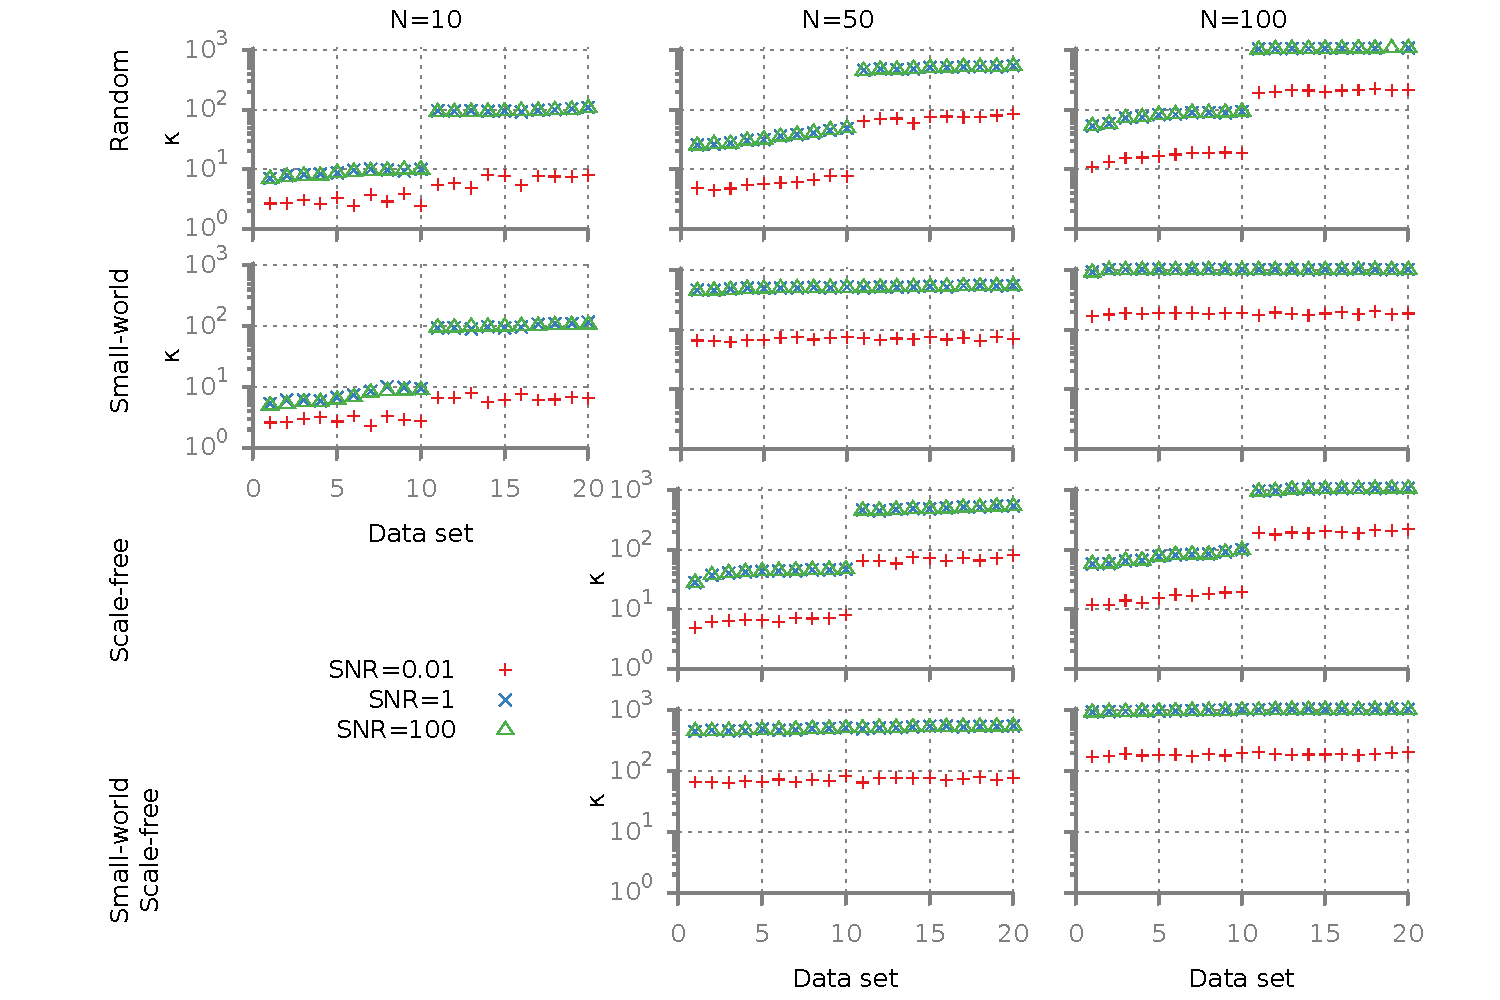
\includegraphics[width=.7\linewidth]{img/data_condition}
\captionsetup{width=.7\textwidth}
\caption{Condition numbers of the response matrices in this benchmark. Three different SNRs were used: $100$, $1$, and $0.01$.  The y-axis shows the condition number $\kappa(\mY)$, and the x-axis shows the number in order of increasing IAA.}
\label{fig:k-data}
\end{figure*}

\subsection{Inference method performance analysis}
\label{sec:analysis-results}
A measure of similarity between the inferred network and the ``true" network used to generate the data is needed to evaluate the performance of inference methods.
% \textcolor{red}{
We here used area under the receiver operating characteristic (AUROC). 
The receiver operating characteristic (ROC) depicts the true-positive rate (TPR), i.e. sensitivity or recall, against the false-positive rate (FPR), i.e. fall-out, as a function of the regularisation parameter for LSCO and Glmnet or the confidence score for RNICO and ARACNe, see the example in Figure \ref{fig:single_performance}.%}

\begin{figure*}[!htb]
\centering
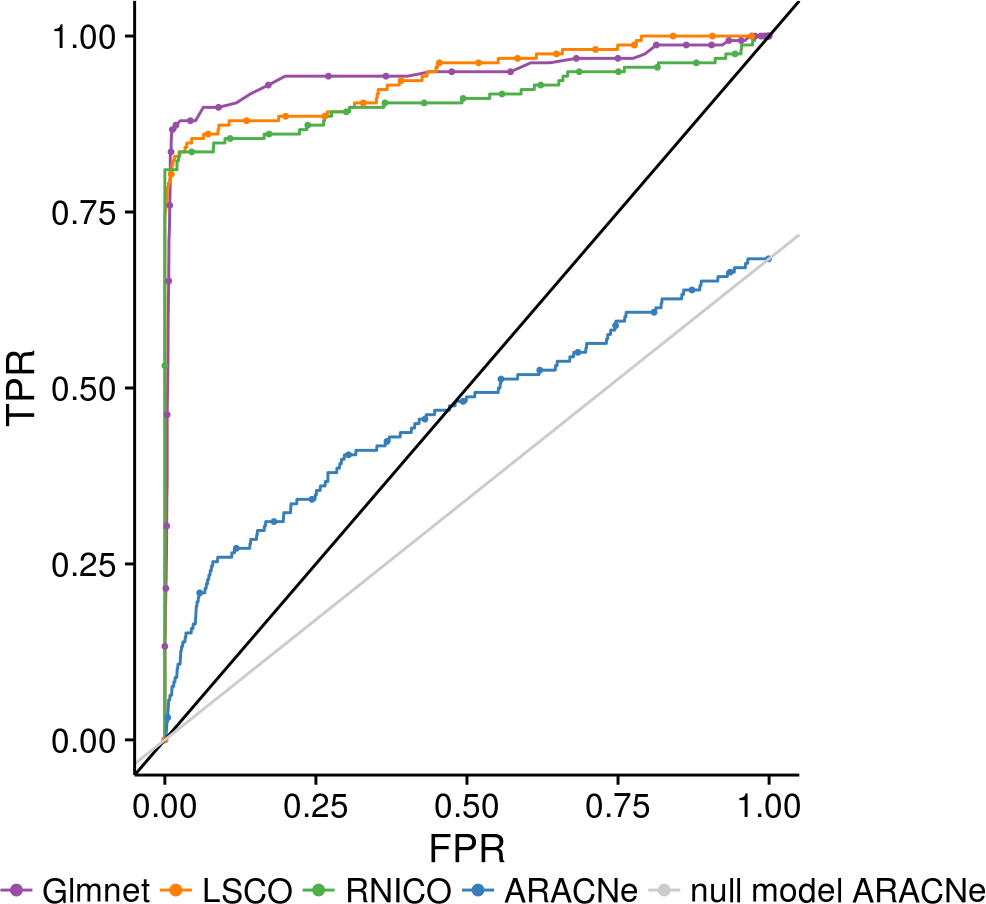
\includegraphics[width=.5\linewidth]{img/ROCcurve.png}
\captionsetup{width=.7\textwidth}
\caption{The ROC curve of four inference methods--Glmnet (\lasso), LSCO, RNICO, and ARACNe--on the Random 50 gene, high IAA, SNR 1 dataset generated by \gs. Note that ARACNe cannot infer self-loops and  therefore has a different null model.}
\label{fig:single_performance}
\end{figure*}

By inferring networks for 100 different values of the regularisation parameter or each confidence score that adds a link we brought the sparsity of the inferred network from an empty network to a full network.
An AUROC of one corresponds to inference of the true network for some regularisation parameter or confidence score with inclusion of all existing links first and then all non-existing ones, while zero corresponds to inclusion of all non-existing links first and then all existing ones such that all networks that can be inferred have the least resemblance to the true network.
% \textcolor{red}{
To compare the four inference methods across the networks and data sets in the benchmark suite, we summarize their AUROC values as bars plots in Figure \ref{fig:performance}. As ARACNe is unable to predict self-loops, we also made a separate benchmark that ignores self-loops entirely (Figure S.3).%}

\begin{figure*}[!htb]
\centering
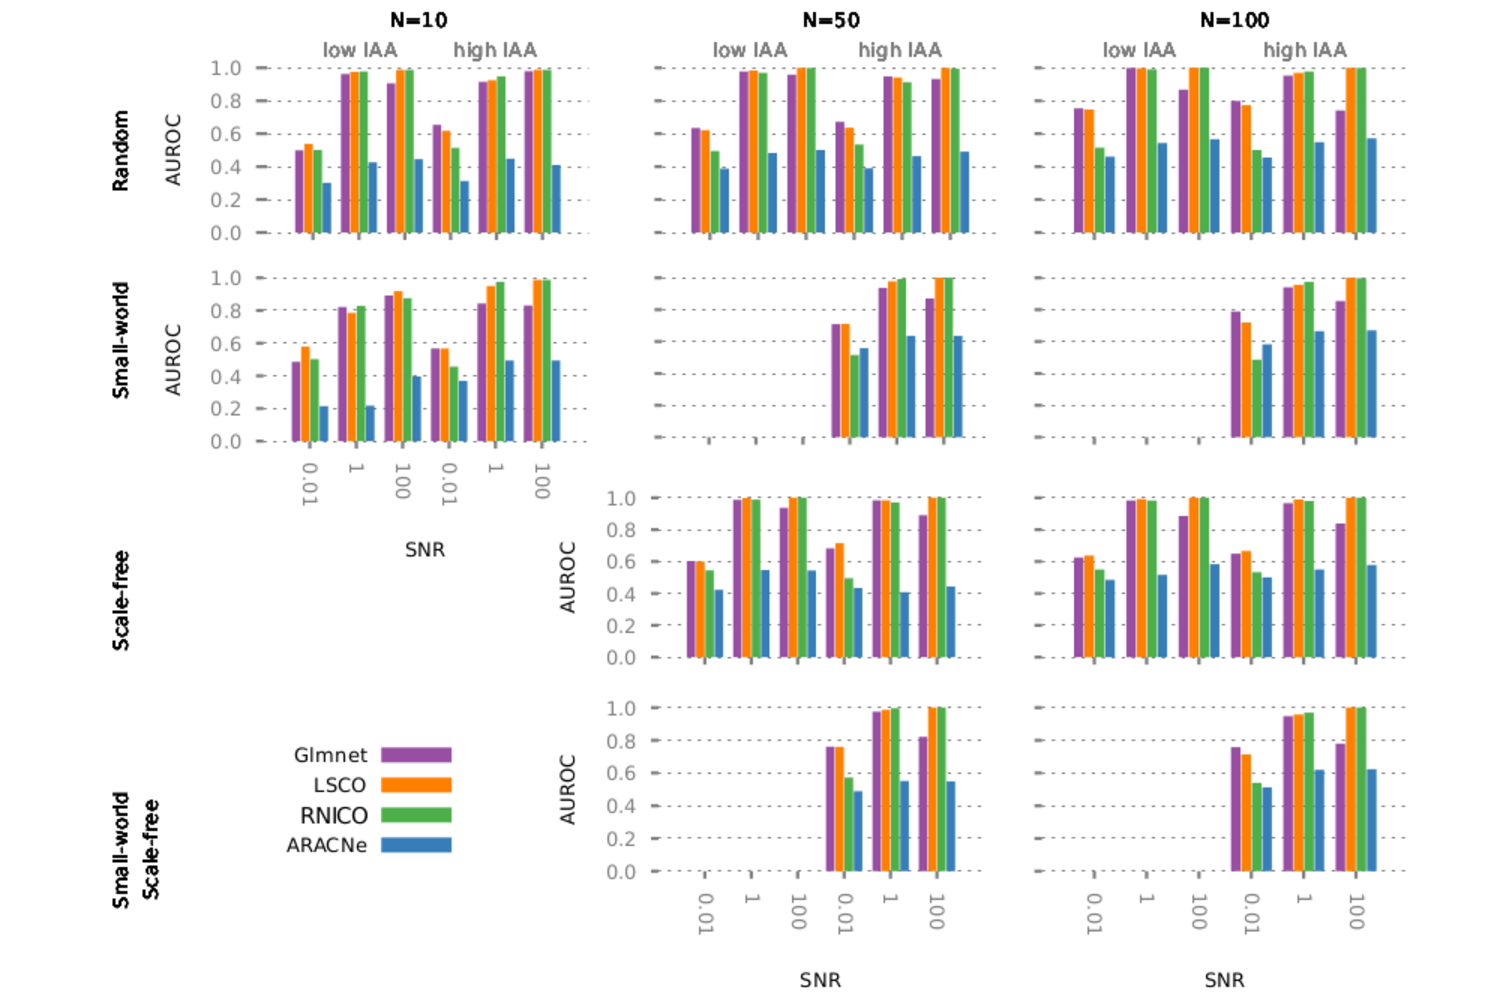
\includegraphics[width=1\linewidth]{img/110117_hasDiag_data_performance}
\captionsetup{width=.7\textwidth}
\caption{Performance of four inference methods -- ARACNe, Glmnet (\lasso), LSCO, and RNICO -- on the benchmark suite  generated by \gs when considering self-loops. The AUROC of an inference method is shown by coloured bars, which are grouped according to IAA degree of the network and SNR of the data (x-axis). The highest and lowest IAA networks were selected among the $20$ networks in each group. Individual ROC curves, MCC plots per sparsity, and density plots per sparsity are available for each condition set in Supplementary Figures, for both considering and not considering self-loops.}
\label{fig:performance}
\end{figure*}

Some major trends can be observed:
\begin{itemize}
\item LSCO and RNICO always give the most accurate networks in cases of SNR 100. The AUROC is almost one and the correct network can in most cases be inferred. RNICO is the preferred method because it can be used to prove the existence of links and provides reliable confidence scores under mild assumptions. To obtain an accurate network using LSCO the correct $\zeta$ value must be selected, while RNICO for a large range of $\zeta$ values will provide accurate networks (Supplementary Figures, MCC panels). However, the correct cut-off to use in RNICO is to set Nordling's confidence score to one, since all links with confidence above one can be proven to exist.

\item Glmnet and ARACNe always fail to infer the correct network when SNR 100, even when LSCO and RNICO succeed, and provide network estimates that are inferior to LSCO and RNICO. This surprising property of Glmnet was previously observed in \cite{Tjarnberg2014}.

\item ARACNe cannot infer self-loops by design, \ie diagonal elements of the interaction matrix. It should therefore be compared to its own null model. Even though it can perform better than random, \ie its null model, in most cases its performance is very poor. ARACNe is clearly outperformed by the other methods in all cases with SNR=1 and 100. For SNR=0.01 it performs similarly to the other methods when not counting self-loops (Figure S.3), but generally close to 0.5 which is the accuracy of random inferences.

\item Glmnet, LSCO, and RNICO have similar AUROC values when SNR= 1, but a good network estimate is given for a narrow range of $\zeta$ values for Glmnet and LSCO, while RNICO yields good estimates for a broad range of values (Supplementary Figures, MCC panels). It is hence easier to obtain a good estimate using RNICO. None of the links can typically be proven to exist using RNICO in this case and the threshold for the confidence score must be selected far below one to get good network estimates.

\item Glmnet is the best method for SNR=0.01 and N=100. In this setting the AUROC values are always below 0.8 however, thus the inferred networks are quite unreliable.

\item In this dataset, changing only the interampatteness gave no clear trend across all methods and property settings.

\item Comparing Figure 3 with Figure S.3, \ie benchmarking with and without considering self-loops, shows that for Glmnet, LSCO, and RNICO this mainly has an effect for SNR=0.01, where the self-loops improve the performance. For N=50 and SNR=0.01, the self-loops alone explain the improvement above random assignment (AUROC=0.5). As expected, ARACNe always scores better when not considering self-loops.

\end{itemize}
\subsection{Benchmark conclusions}
\label{sec:orgheadline8}
The goal of \gs is to provide a common environment for network inference testing and evaluation. We have demonstrated some of its capabilities by generating a benchmark suite of networks and datasets, and used it to analyze the performance of four inference methods.  

It is clear from the benchmarking that mutual information based methods such as ARACNe are generally performing substantially worse than system-optimising methods. This highlights the importance of understanding the system as a whole, which is not achievable by unconnected calculations on the links. ARACNe is further hampered by the fact that it cannot predict self-loops, which are important to bring the system to a stable state, but even if self-loops are ignored its performance is far below the other methods on the two high-SNR settings.
In general, we observed a larger difference in performance in the jump from SNR 0.01 to 1 than from 1 to 100, suggesting a threshold level of noise from which knowledge is recoverable, after which point the noise decrease is less relevant.

Once an algorithm is decided upon, having been vetted against methods of varying strengths and weaknesses, the capability of that choice must be evaluated. Again, our benchmark allowed us to draw the following conclusions:
All methods perform poorly when the SNR is below one because the data simply is not informative enough for network inference.
For high SNRs RNI yields networks that are identical or almost identical to the ``true" network.